\chapter{Access Control Systems}
Access control systems can be broadly categorized into \textit{physical} and \textit{logical} types. 

Physical access control restricts entry to all physical locations, such as buildings or rooms, using methods like keypads, card readers, or biometric scanners.

Logical access control, on the other hand, regulates access to digital resources, such as computer systems or data, using methods like passwords, multi-factor authentication, and authorization policies.

\section{Physical Access Control Examples}
\begin{itemize}
    \item Keypads: Users enter a code to gain access.
    \item Card Readers: Access is granted by swiping or tapping a card.
    \item Biometric Scanners: Access is based on unique biological traits such as fingerprints or iris scans.
    \item Mullion Readers: Slim readers that can be mounted on narrow door frames.
    \item Door Strikes: Electric locks that release the door when triggered by an access control system.
\end{itemize}

\section{Logical Access Control Models}
There are six common logical access control models that you need to be aware of. 
\begin{enumerate}
    \item Discretionary Access Control (DAC) model
    \item Mandatory Access Control (MAC) model
    \item Role-Based Access Control (RBAC) model
    \item Rule-Based Access Control (RuBAC) model
    \item Lattice-Based Access Control (LBAC) model
    \item Attribute-Based Access Control (ABAC) model
\end{enumerate}

The models are ranked purely from an attacker's view-assuming average implementation quality-this is roughly the order from easiest to hardest to compromise:
\textbf{Ranking Summary} \textit{(Easiest →  Hardest):}
DAC →  RBAC →  RuBAC →  ABAC →  LBAC →  MAC

Below is a detailed breakdown of each model:

\section{Discretionary Access Control}
\textit{Discretionary Access Control (DAC)} gives resource owners the ability to manage who has access to their specific resources, such as files and folders. This allows the owner to determine which users or groups can read, write, or execute certain operations on those resources. It is a flexible system where the owner, rather than a central administrator, controls access rights. A more detailed explanation is offered below.

\begin{figure}
    \centering
    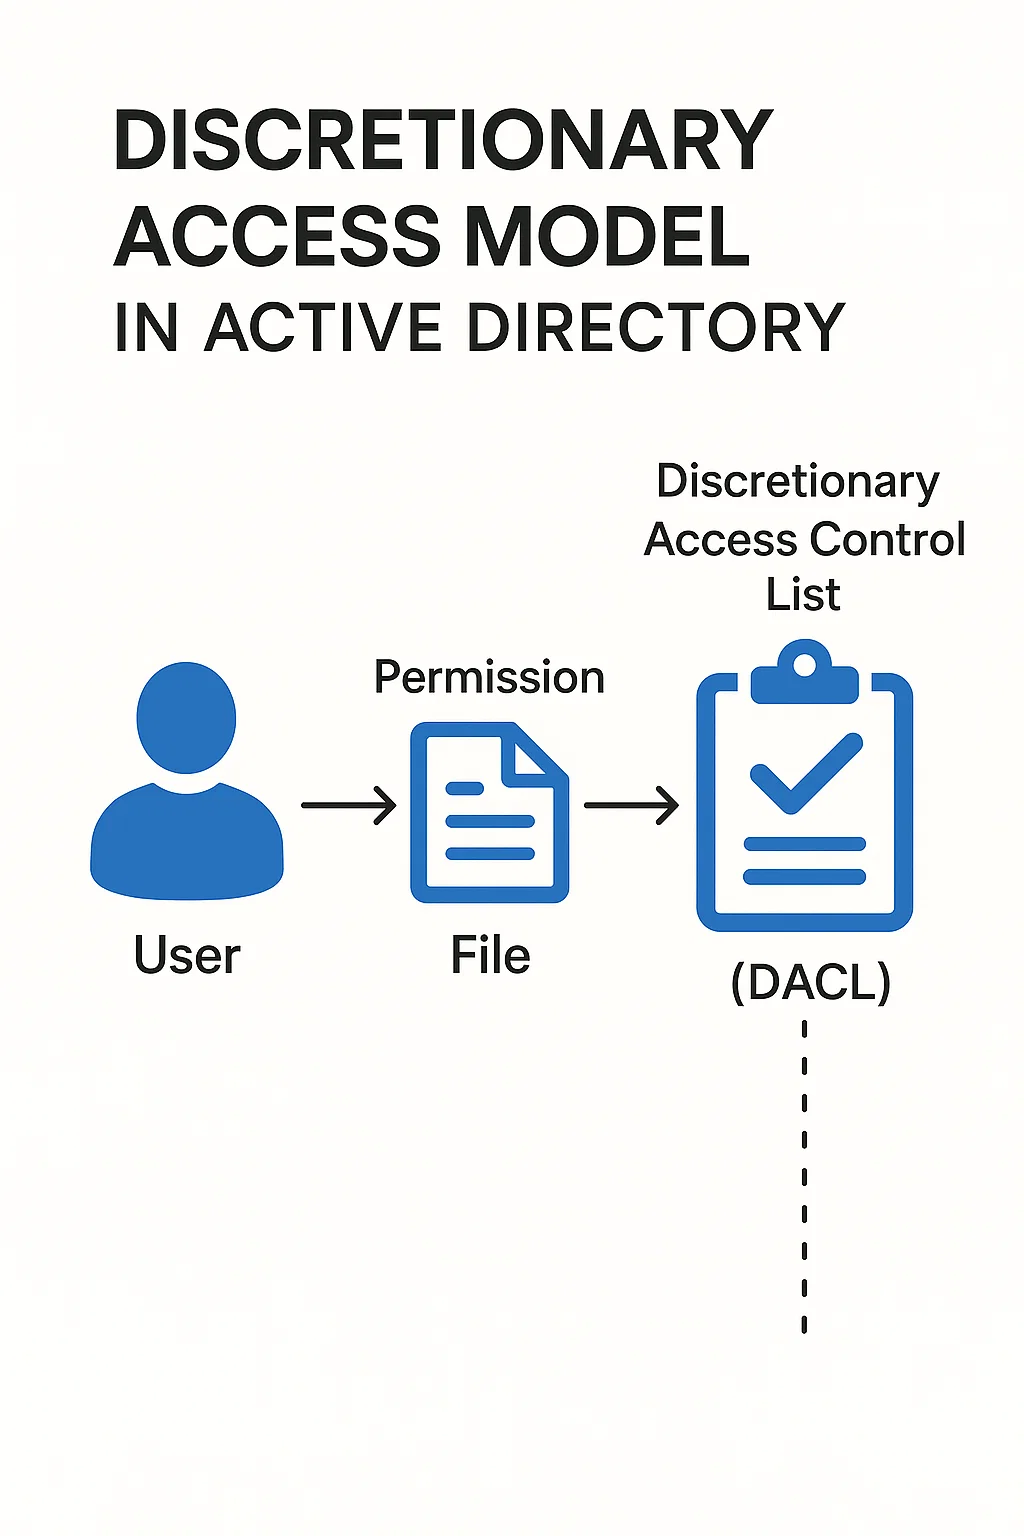
\includegraphics[width=0.75\linewidth]{dac.png}
    \caption{Discretionary Access Control (DAC) model workflow}
    \label{fig:placeholder}
\end{figure}

\subsection{Key Aspects of DAC}
Key aspects of DAC include resource owners setting permissions, flexibility in granting access, and potential vulnerabilities due to human error.

\subsubsection{\textbf{1. Resource Ownership and Permissions:}}
\begin{itemize}
    \item In DAC, the owner of a resource has the power to define access rights for other users.
    \item This includes specifying who can read, write, or execute the resource(s).
    \item Examples include setting permissions on a file in a file system or sharing a Google Doc with specific users.
\end{itemize}
\subsubsection{\textbf{2. Flexibility and User Control:}}
\begin{itemize}
    \item DAC provides flexibility as users can easily adjust permissions based on their needs and collaboration requirements.
    \item Users can grant access to individuals or groups, making it easier to share resources.
    \item This contracts with Mandatory Access Control (MAC) where access is centrally controlled based on security labels.

\end{itemize}
\subsubsection{\textbf{3. Potential Vulnerabilities:}}
\begin{itemize}
    \item The flexibility that DAC provides can also be a source of a vulnerability.
    \item Incorrect permissions can be set by users that can potentially lead to unauthorized access.
    \item Insider threats are a concern, as users with access can potentially misuse it.
    \item Malware can spread more easily if users inadvertently grant access to malicious files.
4. \subsubsection{\textbf{Key Components:}}
\begin{itemize}
    \item Access Control Lists (ACLs): These lists define the permissions associated with a resource.
    \item Permissions and Rights: These specify what actions users can perform on a resource (e.g., read, write, execute).
    \item Resource Owners: These are the users who have the authority to manage access to their resources.
\end{itemize}
\end{itemize}

The core idea is that the individual or entity that owns a particular resource (such as a file, folder, or even an Active Directory object) gets to decide who can interact with it.

How DAC Works
Discretionary Access Control (DAC) is an access control model where the owner of a resource (like a file or folder) has the power to decide who can access it and what they can do with it. This means the owner can grant, revoke, or modify permissions at their discretion. It is a flexible approach, often used in environments where collaboration and sharing of network resources are common.

The Common DAC Workflow
\begin{enumerate}
    \item Resource Ownership: In DAC, each resource such as files, folders, databases) has an owner. This owner is typically the person who created the resource or otherwise designated as the controller.
    \item Permission Assignment: The owner can set permissions for different users and groups, specifying what actions they are allowed to perform on the resource. For example, an owner might grant one user read-only access while giving another user both read and write permissions.
    \item Flexibility and User-Centricity: DAC is known for its flexibility and user-friendliness. Resource owners can easily adjust permissions as needed, making it suitable for collaborative work and dynamic environments.
\end{enumerate}

DAC Attack Vectors
Attack vectors are the methods or pathways through which attackers can gain unauthorized access to a system, network, or application. They exploit vulnerabilities to carry out malicious activities like data theft or system compromise. Essentially, attack vectors are the \textit{"how"} of a cyberattack, while the \textit{"what"} is the target or attack surface. A detailed explanation is offered below.

1. Technical Vulnerabilities
Software Exploits:
Attackers exploit bugs or weaknesses in software, operating systems, and applications to gain access.
Network Exploits:
Attackers target network configurations, network communications protocols, and services to infiltrate systems.
Misconfigurations:
Incorrectly, unsecured systems such as cloud services or Windows security settings can create easy entry points.
Unpatched Vulnerabilities:
Systems with outdated software or security patches are vulnerable to known exploitations.
SQL Injection (SQLi): Attackers manipulate database queries to access or modify sensitive information.
Cross-Site Scripting (XSS): Attackers inject malicious scripts into websites to steal user data or redirect users.

2. Human-Based Vulnerabilities:
Phishing:
Attackers use deceptive emails, messages, or websites to trick users into revealing sensitive information or clicking malicious links. 
Social Engineering:
Attackers manipulate users into divulging information or performing actions that compromise security.
Insider Threats:
Malicious actions by individuals within an organization, such as employees or contractors. 
Compromised Credentials:
Weak or reused passwords, stolen credentials, or compromised accounts can be used to access systems. 
Third-Party Breaches:
Attackers exploit vulnerabilities in a company's third-party vendors to gain access to the company's systems. 

3. Other Attack Vectors:
Ransomware:
Attackers encrypt data and demand a ransom for its release. 

Malware:
Malicious software, such as viruses, worms, and Trojans, can be used to compromise systems. 

Brute-Force Attacks:
Attackers try numerous passwords until they find the correct one. 

DDoS Attacks:
Attackers flood a system with traffic to make it unavailable. 

DAC Attack Vector Mitigation Strategies
To mitigate DAC attack vectors, defenders need to focus on implementing strong security practices such as robust access controls, regular security assessments, and employee training. This includes enforcing strong password policies, using MFA, limiting user privileges, and regularly updating software. Additionally, continuous monitoring, network segmentation, and a comprehensive incident response plan are crucial for identifying and responding to potential attacks. A detailed explanation is offered below.

Implement Strong Access Controls:
\begin{itemize}
    \item Multi-Factor Authentication (MFA): Adding an extra layer of authentication beyond passwords makes it harder for attackers to gain access.
    \item Least Privilege Access: Grant users only the minimum necessary permissions to perform their tasks.
    \item Regular Access Reviews: Periodically review and update user permissions to ensure they are still appropriate.
\end{itemize}

Vulnerability Management:
\begin{itemize}
    \item Regular Security Assessments: Conduct regular vulnerability scans and penetration tests to identify and address weaknesses.
    \item Patch Management: Keep software and systems up-to-date with the latest security patches to address known vulnerabilities.

\end{itemize}

Network Security:
\begin{itemize}
    \item Network Segmentation: Divide the network into smaller, isolated segments to limit the impact of a breach.
    \item Firewalls and Intrusion Detection/Prevention Systems (IDS/IPS): Use these tools to monitor network traffic and block malicious activities.
\end{itemize}

Employee Training:
\begin{itemize}
    \item Cybersecurity Awareness Training: Educate employees about common attack vectors, such as phishing and social engineering, to help identify and avoid threats.
    \item Incident Response Training: Train employees on how to respond to security incidents and report suspicious activities.
\end{itemize}

Continuous Monitoring and Alerting:
\begin{itemize}
    \item Security Information and Event Management (SIEM): Use SIEM tools to collect and analyze security logs for suspicious activities.
    \item Intrusion Detection/Prevention Systems (IDS/IPS): Deploy IDS/IPS to monitor network traffic for malicious activities.
\end{itemize}

Incident Response Plan (IRP):
\begin{itemize}
    \item Develop a Comprehensive Plan: Outline the steps to take in the event of a security breach to minimize damage and ensure a swift recovery.
\end{itemize}

Supply Chain Security:
\begin{itemize}
    \item Assess Vendor Security: Evaluate the security practices of third-party vendors and suppliers.
    \item Secure Third-Party Access: Implement strict access controls for third-party vendors to prevent unauthorized access to your systems.
\end{itemize}

Benefits or RuBAC
Rule-Based Access Control (RuBAC) offers several key benefits, including enhanced security through precise access control, improved scalability, better auditability, and reduced administrative overhead. By implementing RuBAC, organizations can enforce strict access policies, simplify access management, and streamline compliance efforts

\textbf{Precise Access Control:}
RuBAC allows organizations to define rules that dictate who can access specific resources based on various conditions (e.g., time of day, user role, location). This granular control minimizes the risk of unauthorized access and data breaches. 

Reduced Risk of Data Breaches:
By limiting access to only those who need it, RuBAC reduces the potential attack surface and lowers the likelihood of sensitive data falling into the wrong hands. 

Centralized Rule Management:
RuBAC allows for central management of access rules, making it easier to apply policies across different departments, devices, and locations. 

Simplified Onboarding/Offboarding:
Adding or removing access for users is simplified through rule updates, reducing the administrative burden of managing individual permissions. 

Detailed Audit Trails:
Every access decision in RuBAC is based on a rule, providing a clear and auditable trail of user activity. 

Compliance Support:.
The auditability of RuBAC makes it easier to demonstrate compliance with various regulatory and industry standards. 

Centralized Management:
Instead of managing permissions on a user-by-user basis, RuBAC allows for centralized rule management, streamlining administrative tasks.

Automated Rule Updates:
When rules need to be updated, it can often be done centrally, reducing the need for manual adjustments and minimizing the risk of human error. 
Other Benefits:
Improved Operational Efficiency:
By granting users access only to the resources they need, RuBAC can streamline workflows and improve overall operational efficiency. 

Simplified Access Management:
RuBAC simplifies access management by providing a structured and consistent approach to granting and revoking permissions. 

Reduced Costs:
By optimizing resource access and reducing the risk of security incidents, RuBAC can lead to cost savings for the organization.
 


Active Directory uses ACLs, which are lists of \textit{Access Control Entries (ACEs),} to implement DAC. Each ACE specifies which user or group has what level of access (read, write, execute) that particular resource.

\subsubsection{Flexibility and Control}
DAC provides flexibility for users and administrators to manage access to their own data and resources without needing constant IT intervention.

\subsubsection{Potential Security Considerations for Defenders}
While flexible, DAC can be less secure than other access control models (such as \textit{Mandatory Access Control (MAC))} if not managed carefully and properly, as incorrect settings can lead to unintended consequences.

\subsubsection{Abusing Discretionary Access Control (DAC)}
Attackers leverage various entry points, also known as \textit{attack vectors,} to exploit vulnerabilities and gain toehold within a network. These vectors can range from technical flaws such as software backdoors and misconfigurations in systems to human-centric methods such as spearphishing and reuse of passwords.

With DAC, attackers try to manipulate permissions to escalate their privileges or access sensitive data.

Common DAC abuses include, but are not limited to:
\begin{itemize}
    \item Software Vulnerabilities: Exploiting bugs or weaknesses in software to gain initial access.
    \item Misconfigured Systems: Taking advantage of improperly configured systems, such as open network ports or weak access controls.
    \item Phishing: A deception tactic that involves deceiving users into revealing sensitive information through fraudulent emails, attachments, or websites.
    \item Malware: Introducing malicious software to compromise systems and exfiltrate data.
    \item Credential Stuffing: Using stolen usernames and passwords from other breaches to access accounts.
    \item Weak, Default, Exposed, or Reused Passwords: Utilizing easily guessed or reused passwords and default credentials. More often than not, a user will reuse the same password across many various platforms online (e.g., use the same password to log in to banking account and Facebook account).
    \item Social Engineering: Also known as \textit{human hacking,} social engineering attacks aim to manipulate individuals to perform actions that compromise overall security.
    \item Physical Access: Gaining physical access to devices to exploit vulnerabilities or install malware.
\end{itemize}

\subsection{DAC Attack Vectors}
In systems with Discretionary Access Control (DAC), attacker might exploit the following to gain unauthorized access or escalate privileges to laterally move throughout the domain network.

\subsubsection{Abusing Improperly Configured Permissions:}
If permissions are not set correctly, attackers can leverage overly permissive access to escalate their privileges.

\subsubsection{Exploiting Vulnerabilities in Access Control Mechanisms:}
Attackers can find weaknesses in the way access is granted and revoked, allowing them to bypass and evade security control mechanisms.

\subsubsection{Manipulating User Roles and Groups:}
Attackers might try to elevate their access by gaining control of user accounts with higher privileges or by joining privileged groups.

\subsubsection{Bypassing Authentication:}
If authentication mechanisms are weak, attackers can try to bypass and evade them to gain initial access.

\subsubsection{Utilizing Misconfigured Cloud IAM Roles in Active Directory for Cloud:}
In AD cloud-based environments (namely \textit{Azure AD, or AAD),} attackers might exploit overly permissive \textit{Identity and Access Management (IAM)} roles and policies.

\textbf{Example:}
Imagine an attacker who gains access to a user account with limited permissions. If that user has access to a file with overly permissive DAC settings, the attacker might be able to escalate their privileges and gain access to other parts of the restricted network.

\subsection{DAC Attack Vector Mitigation Strategies}
\subsubsection{\textbf{Regular Security Audits:}}
Defenders must regularly review and assess access controls to identify and correct misconfigurations.

\subsubsection{\textbf{Principle of Least Privilege (PoLP):}}
Defenders need to ensure that users and applications only have the minimum necessary permissions, and nothing more than what they're required to have to complete their tasks.

\subsubsection{\textbf{Strong Authentication and Authorization:}}
Defenders must implement authentication and authorization mechanisms to prevent unauthorized access to resources.

\subsubsection{\textbf{Patch Management Cadence:}}
Defenders must adhere to stringent patch management policies and keep systems and software up-to-date with the latest security patches to address known vulnerabilities.

\subsubsection{\textbf{User Education and Awareness:}}
Defenders must train users and staff to recognize and avoid phishing attacks and other social engineering attack tactics.

\subsubsection{\textbf{Implement Access Control Best Practices:}}
Follow industry best practices for setting up and managing access control in your AD environment(s).

\section{Mandatory Access Control (MAC) Model}
\textit{Mandatory Access Control (MAC)} is an access control security mechanism model where access to resources is strictly controlled based on a system-wide security policy defined by a central authority, rather than by individual resource owners. This means users cannot override or change the access permissions set by the central authority, ensuring a high level of security and account scrutiny to prevent unauthorized access. A detailed explanation is offered below.

\subsection{Key Aspects of MAC}
\subsubsection{\textbf{Centralized Policy:}}
Access decisions are made based on a pre-defined security policy enforced by the central authority, not by the users.

\subsubsection{\textbf{Security Labels:}}
Both users and resources are assigned security labels (e.g., classification levels like "Confidential," or "Secret").

\subsubsection{\textbf{Strict Enforcement:}}
Access is granted only when the user's clearance level matches or exceeds the resource's security label.

\subsubsection{\textbf{No User Control:}}
Individual users cannot modify the permissions for their resources, unlike in the Discretionary Access Control (DAC) model.

\subsubsection{\textbf{High Security:}}
MAC is often used in environments requiring high security, such as government, military, and some financial institutions.

\subsubsection{\textbf{Multi-Level Security (MLS):}}
MAC is frequently implemented in MLS systems, which manage data with different security classifications.

\subsection{How MAC Works}
\begin{enumerate}
    \item Central Authority: A security administrator defines the overall security policy, or the user's upper management decides.
    \item User and Resource Classification: Users are assigned security clearance levels, and resources are assigned appropriate security classifications.
    \item Rule Enforcement: The system checks the user's clearance and the resource's classification to determine if access should be granted.
    \item No User Override: Users cannot change the security labels or alter the access rules.
\end{enumerate}

\textbf{Examples of MAC in Use:}
\begin{itemize}
    \item Government and Military: Protecting classified documents and information systems.
    \item Financial Institutions: Securing sensitive financial data and user transactions.
    \item Healthcare: Protecting patient records and medical information.
\end{itemize}

\subsection{MAC Attack Vectors}
Attackers utilize various entry points and attack vectors to bypass Mandatory Access Controls (MAC) systems, aiming to gain that initial toehold into the domain network. Similar to DAC, these methods exploit vulnerabilities in the MAC system's security posture, including technical flaws, human errors, and weaknesses in the implementation of security policies. It is crucial that defenders understand these attack vectors to develop robust security strategies to protect organizational sensitive information and its critical information systems.

\subsubsection{\textit{1. Technical Vulnerabilities:}}
\textbf{Software Exploits:}
Attackers exploit bugs and weaknesses in software applications, operating systems, and network protocols to gain initial access.

\textbf{Unpatched Systems:}
Vulnerabilities in unpatched systems provide readily available entry points for attackers to leverage and exploit.

\textbf{Weak, Default, Exposed, or Reused Passwords:} Stolen or weak passwords, default and reused, or exposed credentials, and improperly stored credentials can be easily exploited if not hardened.

\textbf{Network-based Attacks:}
Attackers can abuse network protocols, such as TCP/IP, to launch attacks like \textit{Man-in-the-Middle (MiTM)} attacks or \textit{Denial of Service (DoS)} attacks.

\textbf{SQL Injection (SQLi) Attack:}
Attackers can inject malicious and arbitrary SQL code into input fields to manipulate database queries and gain unauthorized access to sensitive data.

\textbf{Cross-Site Scripting (XSS) Attack:}
Attackers can also inject malicious scripts into websites to steal users data or hijack user sessions.

\subsubsection{\textit{2. Human-Based Attacks:}}
\textbf{Phishing:}
Attackers impersonate trusted individuals or organizations to trick users into revealing sensitive information such as passwords or account details. 

\textbf{Social Engineering:}
Attackers manipulate users into divulging confidential information or granting access through deception and psychological manipulation. 

\textbf{Insider Threats:}
Malicious or negligent insiders can exploit their access privileges to bypass MAC and access sensitive resources. 

\subsubsection{\textit{3. Supply Chain Attacks:}}
\textbf{Compromised Third-Party Components:}Attackers target third-party vendors or suppliers with weak security to gain access to the main organization's systems. 

\textbf{Malware in Software Updates:}
Attackers can embed malware into software updates, which are then distributed to a wide range of users. 

\subsubsection{\textit{4. Physical Access:}}
\textbf{Physical Security Breaches:}
Attackers can bypass physical security measures to gain access to systems and devices. 

\subsection{MAC Attack Vector Mitigation Strategies}

\subsubsection{\textbf{Reduce Attack Surface:}}
Implement security controls to reduce the number of entry points and vulnerabilities. 

\subsubsection{\textbf{Strong Authentication and Authorization:}}
Enforce strong passwords, multi-factor authentication, and granular access controls. 

\subsubsection{\textbf{Regular Security Audits:}}
Conduct regular security audits to identify and address vulnerabilities. 

\subsubsection{\textbf{Patch Management Cadence:}}
Implement a robust patch management process to quickly address software vulnerabilities. 

\subsubsection{\textbf{Security Awareness Training:}}
Educate users about common attack vectors and best practices for security. 

\subsubsection{\textbf{Incident Response Plan:}}
Develop and test an incident response plan to quickly detect, contain, and recover from attacks. 

\section{Role-Based Access Control (RBAC) Model}
Role-Based Access Control (RBAC) is a security approach that restricts system access based on a user's role within an organization. Instead of assigning permissions directly to individual users, RBAC groups users into roles, and these roles are then granted specific permissions. This approach simplifies access management, enhances security, and promotes compliance by ensuring users only have access to the resources necessary for their job functions, according to cybersecurity and access management companies. A more detailed explanation is offered below.

\subsection{Key Aspects of RBAC}
\begin{itemize}
    \item Users: Individuals who need access to the system. 
    \item Roles: Predefined sets of permissions that define what a user can do within the system. 
    \item Permissions: Specific access rights associated with resources, such as reading, writing, or modifying data. 
\end{itemize}

\subsection{How RBAC Works}
\begin{enumerate}
        \item Define Roles: Identify the different roles within the organization and their corresponding responsibilities. 
        \item Assign Permissions: Grant specific permissions to each role, defining what actions users in that role can perform. 
        \item Assign Users to Roles: Assign users to the appropriate roles based on their job functions. 
\end{enumerate}

\subsection{Benefits of RBAC}
\textbf{Improved Security:}
Restricts access to sensitive data and resources, minimizing the risk of unauthorized access. 

\textbf{Simplified Management:}
Makes it easier to manage user access rights, especially in large organizations. 

\textbf{Enhanced Compliance:}
Helps organizations meet regulatory requirements by providing a structured and auditable access control mechanism. 

\textbf{Increased Efficiency:}
Ensures users have the access they need to perform their jobs, improving overall productivity. 

\textbf{Scalability:}
Easily adaptable to changing organizational structures and user needs. 

\subsection{Example of RBAC In Use}
In a company, a sales representative might be assigned the role of "Sales Rep," which grants them access to customer data and sales reports; however, they might not have access to the company's financial records or HR information, which are managed by other roles.

\subsection{RBAC Entry Points and Attack Vectors}
Attackers utilize various entry points and exploit weaknesses in Role-Based Access Control (RBAC) to compromise systems and gain unauthorized access. Common entry points include vulnerabilities in software, misconfigured systems, and social engineering tactics. RBAC, when poorly implemented or bypassed, can lead to attackers gaining elevated privileges or accessing sensitive data. 

\textbf{Unpatched Software:}
Outdated software and operating systems are prime targets for attackers due to known vulnerabilities. 

\textbf{Misconfigured Systems:}
Improperly configured firewalls, routers, and other security settings can create pathways for attackers to exploit. 

\textbf{Open Ports and Weak Protocols:}
Unsecured ports and outdated protocols can be exploited by attackers to gain access to systems. 

\textbf{Weak Passwords and Credentials:}
Compromised credentials, whether through phishing or brute-force attacks, provide attackers with a direct path into systems. 

\textbf{Phishing and Social Engineering:}
Deceptive emails, messages, or websites designed to trick users into revealing sensitive information or downloading malicious files are common attack vectors. 

\textbf{Malware}:
Viruses, worms, ransomware, and other malware can be introduced through various means, including infected downloads and malicious websites. 

\textbf{APIs:}
Attackers can exploit vulnerabilities in APIs to access sensitive data, disrupt services, or escalate privileges. 

\textbf{Insider Threats:}
Malicious or negligent insiders can pose a significant risk, especially if they have elevated access privileges. 

\textbf{Bypassing RBAC:}
Attackers can exploit weaknesses in RBAC implementation to gain access to resources they should not be authorized to access. 

\textbf{Privilege Escalation:}
Once inside a system, attackers may attempt to escalate their privileges to gain access to more sensitive data or systems.

\textbf{Misconfigured Roles:}
Incorrectly configured roles within RBAC can grant users excessive permissions, allowing them to perform actions beyond their job requirements. 

\textbf{Lack of Least Privilege}:
Failure to adhere to the principle of least privilege, where users are only granted the minimum necessary access, can lead to attackers exploiting excessive permissions. 

User accounts with weak passwords or those compromised through phishing attacks can be used to bypass RBAC and gain unauthorized access. 

\subsection{RBAC Attack Vector Mitigation Strategies}
\textbf{Regular Software Updates:}
Patching software and operating systems promptly is crucial to address known vulnerabilities. 
    
\textbf{Secure Configuration:}
Properly configuring firewalls, routers, and other security systems is essential to prevent attackers from exploiting misconfigurations. 
    
\textbf{Strong Authentication:}
Implementing strong authentication methods, including multi-factor authentication (MFA), can help prevent unauthorized access. 
    
\textbf{User Awareness Training:}
Educating users about phishing, social engineering, and other attack vectors can help them identify and avoid potential threats. 

\textbf{RBAC Implementation:}
Properly implementing RBAC, adhering to the principle of least privilege, and regularly reviewing user roles can help minimize the impact of potential attacks. 

\textbf{Regular Security Audits:}
Conducting regular security audits can help identify vulnerabilities and weaknesses in the system, including RBAC implementations. 

\textbf{Monitoring and Logging:}
Implementing robust monitoring and logging systems can help detect suspicious activity and identify potential attacks. 

\section{Rule-Based Access Control (RuBAC)}
Rule-based access control (RuBAC) is a security model where access to resources is determined by predefined rules and conditions, rather than by individual user identities or roles. These rules specify which users or groups can access specific resources based on various attributes, environmental conditions, or other criteria. A more detailed explanation is offered below.

Key Concepts:
Rules:
.
These are the core of RBAC. They are logical statements that define access conditions. For example, a rule might state "Users in the 'Finance' department can access the 'Payroll' folder, but only during business hours". 
Attributes:
.
RBAC relies on attributes associated with users, resources, and the environment to evaluate access requests. Examples include user roles, department, time of day, location, device type, or even specific data within a resource. 
Access Decisions:
.
When a user tries to access a resource, the system evaluates the request against the defined rules. If the user's attributes and the resource attributes meet the criteria specified in the rules, access is granted. Otherwise, access is denied. 
How it Works:
1. Rule Definition:
.
Administrators define rules that specify which users or groups can access specific resources based on various conditions. 
2. Attribute Evaluation:
.
When a user attempts to access a resource, the system collects relevant attributes associated with the user, the resource, and the environment. 
3. Rule Enforcement:
.
The system compares the collected attributes against the predefined rules. 
4. Access Control:
.
Based on the rule evaluation, the system either grants or denies access to the resource. 
Example:
Imagine a company with a database containing sensitive financial information. They might implement RBAC with the following rules: 
Rule 1: "Users with the 'Finance' role can access the 'Financial Data' table." 
Rule 2: "Users with the 'HR' role can access the 'Employee Salaries' table." 
Rule 3: "Users with the 'Marketing' role cannot access either table." 
When a user from the 'Finance' department attempts to access the 'Financial Data' table, the system will evaluate their role against the rules. Since Rule 1 matches their attributes, they will be granted access. Conversely, a user from the 'Marketing' department attempting to access the same table will be denied access because Rule 3 will prevent it. 
Advantages of RBAC:
Granular Control:
RBAC allows for fine-grained access control, enabling administrators to define very specific rules for access. 
Flexibility and Scalability:
RBAC is more flexible than role-based access control (RBAC) as it allows for dynamic adjustments to access based on changing conditions. 
Reduced Administrative Burden:
Once the rules are defined, the system automatically manages access, reducing the need for manual permission management. 
Improved Security:
RBAC can help prevent unauthorized access to sensitive resources by implementing strict access controls. 

\subsection{RuBAC Attack Vectors}
Attack vectors are the pathways attackers use to exploit vulnerabilities and gain unauthorized access to systems. For attackers using rule-based access control, entry points can include exploiting weak or misconfigured rules, bypassing access controls through privilege escalation, or leveraging social engineering to manipulate legitimate users into granting unauthorized access. A more detailed explanation is offered below.

Entry Points for Attackers Exploiting Rule-Based Access Control:
Exploiting Weak or Misconfigured Rules:
.
Attackers can identify and exploit overly permissive or poorly defined access control rules. This could involve rules that grant excessive privileges to certain users or roles, or rules that are not adequately updated to reflect changing system requirements. 
Bypassing Access Controls:
.
Attackers may attempt to bypass access control mechanisms altogether, such as by finding vulnerabilities in the underlying system that allow them to bypass the rule-based system. They may also try to escalate their privileges through techniques like SQL injection or other forms of code injection. 
Social Engineering:
.
Attackers can manipulate legitimate users into granting them unauthorized access. This could involve phishing attacks to steal credentials, tricking users into running malicious software, or exploiting trust relationships to gain access to systems or data. 
Insider Threats:
.
Attackers may be able to exploit existing access rights, or use their position of trust within an organization to gain unauthorized access, potentially bypassing the rule-based system entirely. 
Zero-day Exploits:
.
Attackers may be able to exploit vulnerabilities in the access control system itself, or in the underlying operating system or applications, that are previously unknown (zero-day) to gain access. 
Attack Vectors in Rule-Based Access Control:
Exploiting Vulnerabilities:
Attackers may exploit vulnerabilities in the software or hardware that implements the rule-based access control system. This could involve vulnerabilities in the access control engine itself, or in the underlying operating system or applications that the access control system relies on. 
Compromising Credentials:
Attackers may try to obtain legitimate user credentials through various means, such as phishing, malware, or data breaches. Once they have valid credentials, they can use them to access systems and data based on the rules defined for that user. 
Abusing Existing Permissions:
Attackers may attempt to abuse existing permissions granted to legitimate users. This could involve using stolen or compromised credentials, or exploiting situations where users have unnecessarily broad permissions, according to Palo Alto Networks. 
Bypassing Security Measures:
Attackers may attempt to bypass security measures implemented by the rule-based access control system, such as multi-factor authentication or encryption. 
In essence, attackers will try to find the weakest link in the security chain. This could be a poorly configured rule, a vulnerable piece of software, or a trusting user who can be tricked into revealing their credentials or granting access. 




 
 

 


Information Security Access Controls
Access Control Concepts
Policies, Models, and Mechanisms of Access Control

Temporal Constraints
Access Control Workflow
Chinese Wall